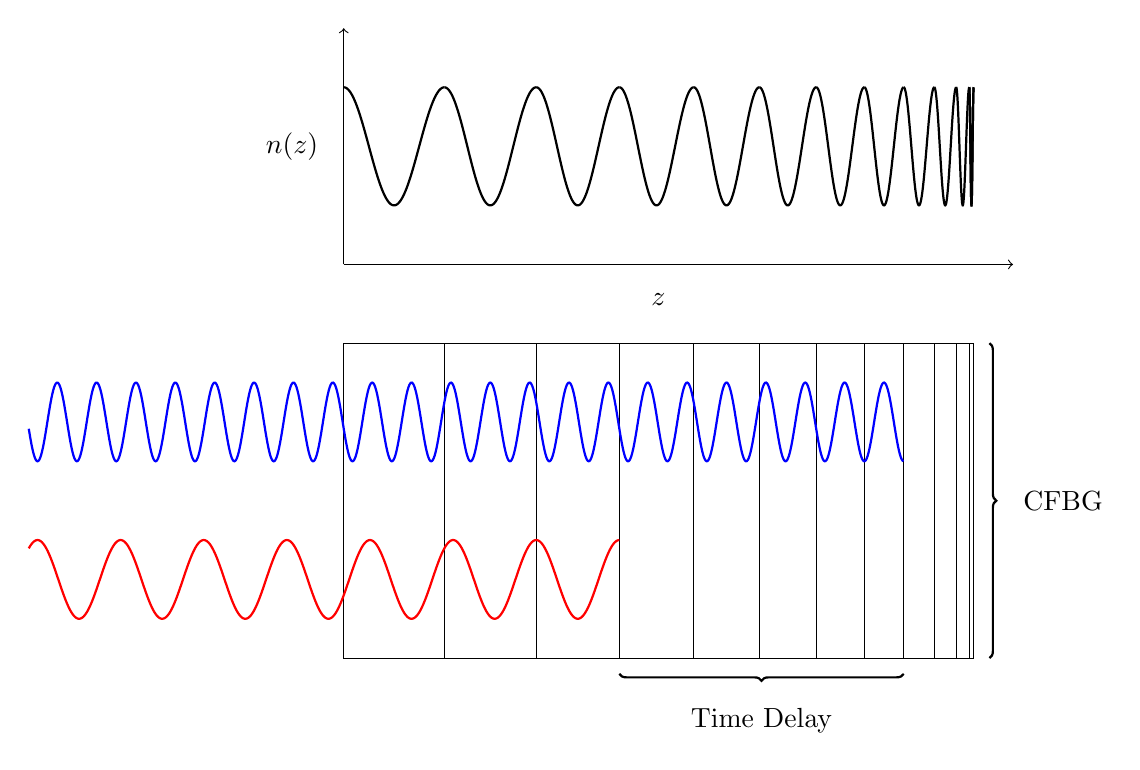
\begin{tikzpicture}
\draw (4,0) -- (12,0) -- (12,4) -- (4,4) -- cycle;
\foreach \i in {1,...,12}
  \draw (12 - 1/18*\i*\i,0) -- (12 - 1/18*\i*\i,4);
%\foreach \i in {0,...,12}
%  \draw [dashed] (12 - 1/18*\i*\i,4) -- (12 - 1/18*\i*\i,8);
\draw [domain=0:(12-16/18), samples=1000, blue, thick] plot (\x, {-0.5*cos(4*pi*(\x-(12-25/18)) r) + 3});
\draw [domain=0:(12-81/18), samples=500, red, thick] plot (\x, {0.5*cos(2*pi*36/38*(\x-(12-100/18)) r) + 1});

\draw [thick, decoration={brace, mirror, raise=0.2cm}, decorate] (7.5,0) -- (100/9,0)
node [pos=0.5,anchor=north,yshift=-0.5cm] {Time Delay};
\draw [thick, decoration={brace, mirror, raise=0.2cm}, decorate] (12,0) -- (12,4)
node [pos=0.5,anchor=west,xshift=0.5cm] {CFBG};

\draw [->] (4,5) -- (12.5,5)
node [pos=0.47,anchor=north,yshift=-0.25cm] {$z$};
\draw [->] (4,5) -- (4,8)
node [pos=0.5,anchor=east,xshift=-0.2cm] {$n(z)$};
\foreach \i in {0,...,12}
  \draw [domain=(12-\i*\i/18):(12-(\i-1)*(\i-1)/18), samples=100, black, thick] plot (\x, {3/4*cos(2*pi*36/(4*\i-2)*(\x-(12-\i*\i/18)) r) + 6.5});
\end{tikzpicture}